\documentclass[11pt]{article}
\usepackage[margin=1in]{geometry}
\usepackage{graphicx}
\usepackage{booktabs}
\usepackage{amsmath}
\usepackage{hyperref}
\hypersetup{colorlinks=true, linkcolor=blue, urlcolor=blue, citecolor=blue}
\usepackage{caption}
\graphicspath{{../figures/}}

\title{Do Natural-Language Autoencoders and Sparse Autoencoders Agree?\\
       A Pilot Comparison on Qwen2.5-7B}
\author{Steven Hou}
\date{July 2026}

\begin{document}
\maketitle

\begin{abstract}
Two families of unsupervised method now claim to explain what a language model
represents in its residual stream, in completely different media. A
\emph{sparse autoencoder} (SAE) decomposes an activation into a sparse
overcomplete code of learned features. A \emph{natural-language autoencoder}
(NLA) verbalizes the \emph{same} activation into free-text English and is
trained so the description alone suffices to reconstruct the vector. Because the
two are trained independently, with different objectives and output spaces, we
can ask a convergent-validity question: on the same activations, do they recover
the same structure? Using the open NLA release for \texttt{Qwen2.5-7B-Instruct}
and an open SAE trained on the same model, we compare them on 216
residual-stream token activations. We find clear agreement. Tokens sharing an
SAE feature are described ${\approx}79\%$ more similarly by the NLA than random
token pairs (cosine lift $+0.189$ over a $0.240$ baseline; $88\%$ of $522$
features positive; a shuffled control at $+0.0006$). Global pairwise-similarity
structure also tracks (Spearman $\rho = 0.213$ vs a shuffled control of
$-0.018$). Both are faithful autoencoders (median reconstruction cosine $0.90$
SAE decoder, $0.92$ NLA reconstructor). This is a small pilot---one model, one
layer, 216 tokens---but it is direct evidence that the structure these methods
surface lives in the model, not the method.
\end{abstract}

\section{Introduction}
Mechanistic interpretability has converged on the residual stream as the object
to explain, and on \emph{autoencoding} as the method: learn a map from an
activation to a human-legible representation and back, and use reconstruction
error to certify that the legible form kept the content. Two such methods have
very different codomains. \textbf{SAEs} map an activation
$h \in \mathbb{R}^d$ to a sparse nonnegative code over an overcomplete
dictionary; each active coordinate is a ``feature.'' \textbf{NLAs} map $h$ to a
short English description via a fine-tuned \emph{activation verbalizer} (AV) and
back via an \emph{activation reconstructor} (AR), trained so the words alone
recover $h$.

Both are unsupervised and validated by reconstruction, but they decompose the
stream into different things: a discrete sparse code vs a paragraph of English.
If both recover something real, their outputs should \emph{agree}. If each is
largely an artifact of its own inductive bias, their outputs should be
uncorrelated once we control for chance. This paper runs that test---possible
only recently, since an open NLA release
(\href{https://github.com/kitft/natural_language_autoencoders}{kitft},
accompanying Anthropic's NLA work) ships AV/AR checkpoints for
\texttt{Qwen2.5-7B-Instruct}, and an open SAE for the same model is available
(\href{https://huggingface.co/andyrdt/saes-qwen2.5-7b-instruct}{\texttt{andyrdt/saes-qwen2.5-7b-instruct}}).

\section{Setup}
\textbf{Target model.} \texttt{Qwen/Qwen2.5-7B-Instruct} (28 layers, $d=3584$).

\textbf{NLA.} \texttt{kitft/nla-qwen2.5-7b-L20-av}/\texttt{-ar}. The NLA reads
``layer 20'' $=$ HF \texttt{hidden\_states[21]} (output of block 20). The AV
injects the activation as one token embedding (L2-renormalized to
$\text{injection\_scale}=150$) into a fixed prompt and greedily autoregresses an
\texttt{<explanation>}; it is served with SGLang via \texttt{input\_embeds}. The
AR gives a reconstruction cosine.

\textbf{SAE.} \texttt{andyrdt/saes-qwen2.5-7b-instruct},
\texttt{resid\_post\_layer\_19}, trainer 0: a BatchTopK SAE, dictionary size
$131{,}072$, $k=32$, inference threshold $3.51$.
\texttt{resid\_post\_layer\_19} $=$ HF \texttt{hidden\_states[20]} (output of
block 19).

\textbf{Layer alignment.} The methods read \emph{adjacent} points: NLA at
\texttt{hidden\_states[21]}, SAE at \texttt{hidden\_states[20]}---one block
apart. We extract both in one forward pass and feed each its native layer. The
offset is a confound (\S\ref{sec:lim}).

\textbf{Data.} 36 short English paragraphs over ${\sim}18$ topics. Per paragraph
we take up to 6 evenly spaced token positions, skipping the first 12 and any
position with residual norm outside $[30,300]$. This yields $N=216$ activations.

\section{Method}
For each token we obtain, from the same forward pass: an NLA description $t_i$
(from the AV at \texttt{hidden\_states[21]}); an SAE code
$f_i \in \mathbb{R}_{\ge 0}^{131072}$ (at \texttt{hidden\_states[20]}); and the
two reconstruction cosines $\cos(h_i, \mathrm{dec}(f_i))$ and
$\cos(h_i, \mathrm{AR}(t_i))$. We embed each $t_i$ with
\texttt{all-MiniLM-L6-v2} (mean-pooled, normalized) to $e_i \in \mathbb{R}^{384}$
and define $S^{\text{text}}_{ij}=\langle e_i,e_j\rangle$ and
$S^{\text{sae}}_{ij}=\cos(f_i,f_j)$. All comparisons are label-free.

\textbf{(A) Feature-conditioned NLA consistency.} For each SAE feature firing on
$\ge 3$ of the 216 tokens (522 features), with firing set $T_f$,
\[
\mathrm{lift}(f) = \operatorname*{mean}_{i<j \in T_f} S^{\text{text}}_{ij}
                   \;-\; \underbrace{\operatorname*{mean}_{i<j}
                   S^{\text{text}}_{ij}}_{\text{baseline } b}.
\]
We report mean lift, fraction positive, and a shuffled control that permutes the
NLA embeddings across tokens ($\approx 0$).

\textbf{(B) Similarity-structure agreement.} Spearman rank correlation between
$S^{\text{text}}$ and $S^{\text{sae}}$ over all $\binom{216}{2}=23{,}220$ pairs,
with a permuted control.

\textbf{(C) Fidelity.} Median SAE decoder cosine vs median NLA AR cosine.

\section{Results}
\begin{figure}[t]\centering
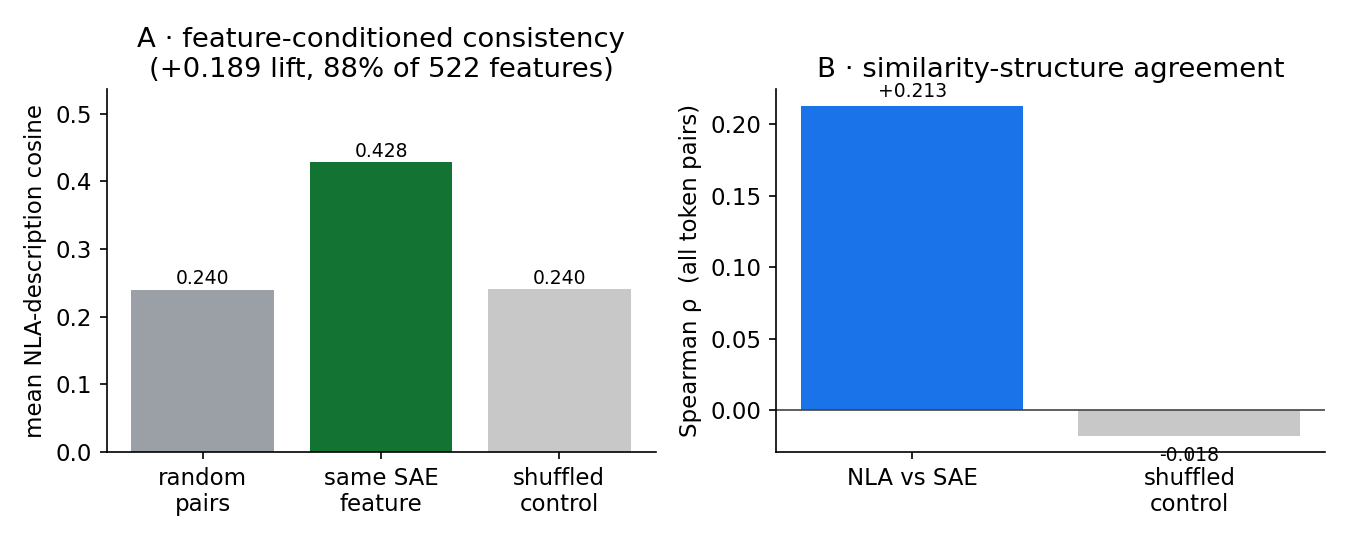
\includegraphics[width=\linewidth]{fig_agreement.png}
\caption{The two agreement tests. Left: conditioning on a shared SAE feature
raises expected NLA-description similarity from $0.240$ to $0.428$; the shuffled
control returns to baseline. Right: NLA and SAE similarity geometries correlate
($\rho=0.213$) while the shuffled control is $\approx 0$.}
\end{figure}

\begin{table}[t]\centering
\begin{tabular}{@{}lll@{}}
\toprule
Test & Result & Shuffled control \\ \midrule
A $\cdot$ feature-conditioned consistency & lift $+0.189$; $88\%$ of 522 feats $+$ & $+0.0006$ \\
B $\cdot$ structure agreement & Spearman $\rho=0.213$ & $-0.018$ \\
C $\cdot$ fidelity (median cosine) & SAE $0.896$ / NLA AR $0.922$ & --- \\ \bottomrule
\end{tabular}
\caption{The methods agree far beyond chance. Test A is the strongest signal;
Test B is a weaker but clearly positive global correlation.}
\end{table}

\begin{figure}[t]\centering
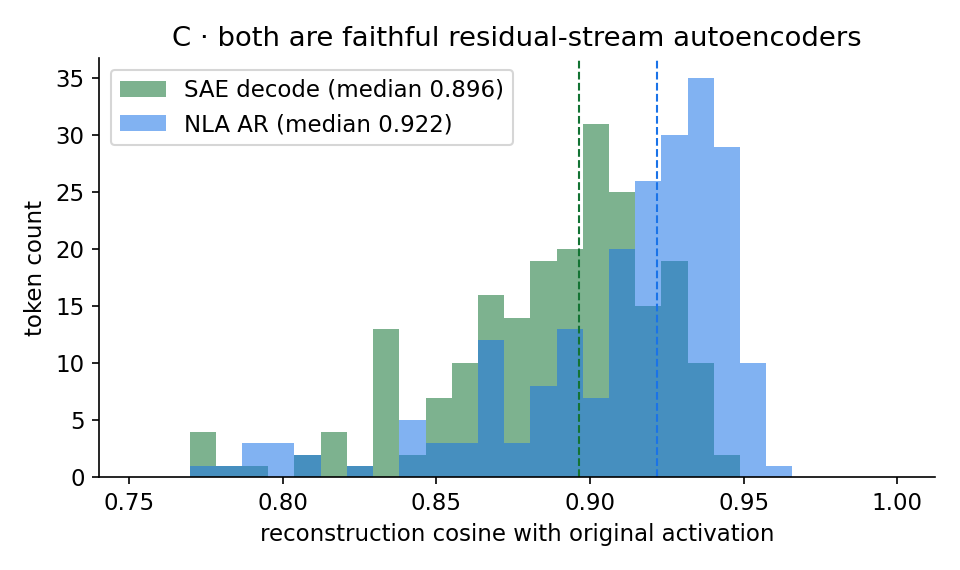
\includegraphics[width=0.72\linewidth]{fig_fidelity.png}
\caption{Both round-trips preserve ${\sim}90\%$ of the activation direction, so
neither method agrees by discarding the content it interprets.}
\end{figure}

Topic-concentrated SAE features are described by the NLA---which never saw the
SAE---as the same subject: feature \#87467 (12 tokens) as biology/cellular
respiration; \#78345 as the Amazon rainforest; \#30775 as geology/earthquakes;
\#106527 as winemaking; \#121136 as contract law; \#118684 as the Fourth
Amendment. The most \emph{frequent} SAE features are instead syntactic (e.g.\
sentence-final periods across every topic); these contribute ${\approx}0$ to
Test A, so the $+0.189$ lift is if anything conservative.

\section{Limitations}\label{sec:lim}
This is a pilot. (i) \textbf{Scale}: $N=216$ tokens, 36 short paragraphs. (ii)
\textbf{One-block layer offset}: NLA at \texttt{hidden\_states[21]}, SAE at
\texttt{[20]}; no open SAE exists at the NLA's exact layer. The offset can both
attenuate real agreement and inflate it via shared information. (iii)
\textbf{Similarity proxy}: MiniLM cosine defines ``similar descriptions''; a
different embedder shifts magnitudes (controls guard against spurious structure,
not embedder bias). (iv) \textbf{Controls are single permutations}, not full
permutation-test $p$-values. (v) \textbf{Single model, single sparsity}
($k=32$). (vi) The qualitative feature$\to$token grouping is rebuilt post-hoc
from each token's top-20 features; metrics use the full on-device active sets.
We claim only that the methods \emph{covary} far beyond chance---not that either
is ``correct'' nor that they are interchangeable.

\section{Discussion}
The result is a convergent-validity signal: two decoders trained with unrelated
objectives---one a sparse code, one English---place activations in agreeing
arrangements. When independent methods agree, the parsimonious explanation is
that the structure is a property of the model, not of either method's bias. This
is mild evidence that SAE features track meaningful directions and that NLA
verbalizations are not free-associative confabulation. The gap between the
strong Test A and the modest Test B is expected: sharing a \emph{specific}
feature is a strong local statement, whereas a \emph{global} rank correlation
mixes features of very different frequency across a layer offset.

\section{Future work}
Scale to 1--2k tokens with per-feature confidence intervals and a permutation
$p$-value; remove the layer confound with a same-layer SAE (or use layer 23 as a
controlled opposite offset); sweep SAE sparsity ($k=32/64/128/256$); test
cross-embedder robustness and compare NLA text against SAE auto-interp labels;
repeat on the other open NLA targets (Gemma-3-12B/27B, Llama-3.3-70B).

\section*{Reproducibility}
Runs serverlessly on \href{https://modal.com}{Modal} on one H100
(${\sim}10$ min, ${\approx}\$0.70$, within the monthly free credits). See the
repository for \texttt{code/run.py}, \texttt{code/probe.py}, and raw outputs.

\begin{thebibliography}{9}
\bibitem{nla} \emph{Natural Language Autoencoders Produce Unsupervised
Explanations of LLM Activations}. Transformer Circuits, 2026.
\url{https://transformer-circuits.pub/2026/nla/};
code \url{https://github.com/kitft/natural_language_autoencoders}.
\bibitem{sae} \texttt{andyrdt/saes-qwen2.5-7b-instruct}.
\url{https://huggingface.co/andyrdt/saes-qwen2.5-7b-instruct}.
\bibitem{batchtopk} Bussmann, Leask, Nanda. \emph{BatchTopK Sparse
Autoencoders}. arXiv:2412.06410, 2024.
\bibitem{gemmascope} Lieberum et al. \emph{Gemma Scope: Open Sparse Autoencoders
Everywhere All At Once on Gemma 2}. arXiv:2408.05147, 2024.
\bibitem{sbert} Reimers, Gurevych. \emph{Sentence-BERT}. arXiv:1908.10084, 2019.
\bibitem{autointerp} Bills et al. \emph{Language models can explain neurons in
language models}. OpenAI, 2023.
\bibitem{qwen} Qwen Team. \emph{Qwen2.5}, 2024.
\url{https://huggingface.co/Qwen/Qwen2.5-7B-Instruct}.
\end{thebibliography}

\end{document}
